\documentclass{chi-ext}

\usepackage{tikz}
\usepackage{verbatim}
%\usepackage[active,tightpage]{preview}
%\PreviewEnvironment{tikzpicture}

\usepackage{graphicx}   % for EPS use the graphics package instead
\usepackage{balance}    % useful for balancing the last columns
\usepackage{bibspacing} % save vertical space in references
\usepackage{paralist}
\usepackage{pgf}
\usetikzlibrary{arrows,automata}
\usepackage[latin1]{inputenc}

\begin{document}

%-----------------------------------------------------
%TEMPLATE: keep at top
\begin{figure}
  \begin{center}
\begin{tikzpicture}

%ADD stuff HERE

\end{tikzpicture}
  \caption{Sample diagram.}
  \label{fig:sample}
    \end{center}
\end{figure}

%-----------------------------------------------------
%SQUARE WAVE 
\begin{figure}
  \begin{center}
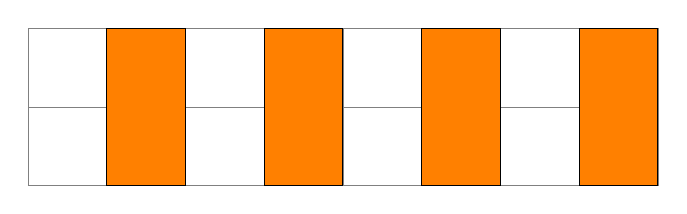
\begin{tikzpicture}

\draw[step=1cm,gray,very thin] (0,0) grid (8,2);
%\draw[thick] (-1,0) -- (0,0);
%\draw[thick] (0,0) -- (1,0);
%\draw[thick] (1,0) -- (1,2);
%\draw[thick] (1,2) -- (2,2);
%\draw[thick] (2,2) -- (2,0);
%\draw[thick] (2,0) -- (4,0);
%\draw[thick] (4,0) -- (4,2);
%\draw[thick] (4,2) -- (5,2);
%\draw[thick] (5,2) -- (5,0);
%\draw[thick] (5,0) -- (7,0);
%\draw[thick] (7,0) -- (7,2);
%\draw[thick] (7,2) -- (8,2);
%\draw[thick] (8,2) -- (8,0);
\filldraw[fill=orange, draw=black] (1,0) rectangle (2,2);
\filldraw[fill=orange, draw=black] (3,0) rectangle (4,2);
\filldraw[fill=orange, draw=black] (5,0) rectangle (6,2);
\filldraw[fill=orange, draw=black] (7,0) rectangle (8,2);


\end{tikzpicture}
  \caption{Sample diagram.}
  \label{fig:sample}
    \end{center}
\end{figure}
%-----------------------------------------------------
%CYCLE w/ NODES
\begin{figure}
  \begin{center}
\begin{tikzpicture}

\def \n {5}
\def \radius {3cm}
\def \margin {8} % margin in angles, depends on the radius

\foreach \s in {1,...,\n}
{
  \node[draw, circle] at ({360/\n * (\s - 1)}:\radius) {$\s$};
  \draw[->, >=latex] ({360/\n * (\s - 1)+\margin}:\radius) 
    arc ({360/\n * (\s - 1)+\margin}:{360/\n * (\s)-\margin}:\radius);
}
\end{tikzpicture}
  \caption{A simple diagram of a cycle.}
  \label{fig:cycle}
    \end{center}
\end{figure}

%-----------------------------------------------------
%3x8 GRID
\begin{figure}
  \begin{center}
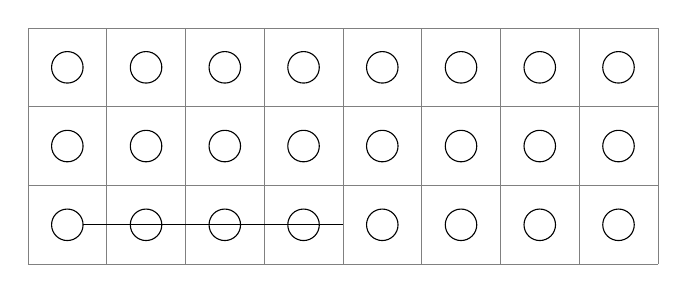
\begin{tikzpicture}

\draw[step=1cm,gray,very thin] (0,0) grid (8,3);
\draw (0.7,0.5) -> (4,0.5);
\draw (0.5,0.5) circle (0.2cm); \draw (0.5,1.5) circle (0.2cm); \draw (0.5,2.5) circle (0.2cm); 
\draw (1.5,0.5) circle (0.2cm); \draw (1.5,1.5) circle (0.2cm); \draw (1.5,2.5) circle (0.2cm); 
\draw (2.5,0.5) circle (0.2cm); \draw (2.5,1.5) circle (0.2cm); \draw (2.5,2.5) circle (0.2cm); 
\draw (3.5,0.5) circle (0.2cm); \draw (3.5,1.5) circle (0.2cm); \draw (3.5,2.5) circle (0.2cm); 
\draw (4.5,0.5) circle (0.2cm); \draw (4.5,1.5) circle (0.2cm); \draw (4.5,2.5) circle (0.2cm); 
\draw (5.5,0.5) circle (0.2cm); \draw (5.5,1.5) circle (0.2cm); \draw (5.5,2.5) circle (0.2cm); 
\draw (6.5,0.5) circle (0.2cm); \draw (6.5,1.5) circle (0.2cm); \draw (6.5,2.5) circle (0.2cm); 
\draw (7.5,0.5) circle (0.2cm); \draw (7.5,1.5) circle (0.2cm); \draw (7.5,2.5) circle (0.2cm); 

\end{tikzpicture}
  \caption{A grid of buttons, LED lights and vibrating motors.}
  \label{fig:sample}
    \end{center}
\end{figure}

%-----------------------------------------------------
% simple automata
\begin{figure}
  \begin{center}
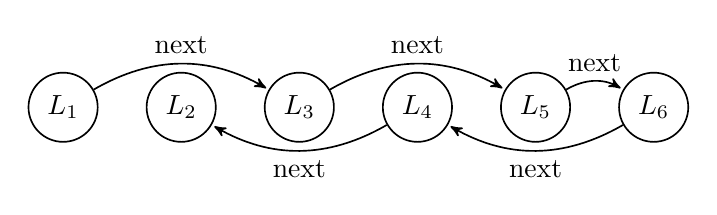
\begin{tikzpicture}[->,>=stealth',shorten >=1pt,auto,node distance=1.5cm, minimum size=6pt, semithick]
	\tikzstyle{every state}=[fill=white,draw=black,text=black]
	\node[state] (1) {$L_1$};
	\node[state] (2) [right of=1] {$L_2$};
	\node[state] (3) [right of=2] {$L_3$};
	\node[state] (4) [right of=3] {$L_4$};
	\node[state] (5) [right of=4] {$L_5$};
	\node[state] (6) [right of=5] {$L_6$};
	%\node[state] (7) [right of=6] {$L_7$};
	%\node[state] (8) [right of=7] {$L_8$};
	
	\path (1) edge [bend left] node {next} (3);
	\path (3) edge [bend left] node {next} (5);
	\path (5) edge [bend left] node {next} (6);
	
	\path (6) edge [bend left] node {next} (4);
	\path (4) edge [bend left] node {next} (2);

\end{tikzpicture}
  \caption{Simple activation pattern for a 1D array of LED lights.}
  \label{fig:sample}
    \end{center}
\end{figure}



\end{document}
